\documentclass{article}
\usepackage{graphicx} % Required for inserting images

\usepackage{auto-pst-pdf} % Enable PSTricks with pdflatex
% If using Overleaf, the -shell-escape flag is already enabled by default for auto-pst-pdf to work
\usepackage{pst-eucl} % Euclidean geometry

\usepackage{tikz} % ChatGPT likes this for drawing some things
\usetikzlibrary{calc,intersections}

\usepackage{mathtools}

\usepackage{hyperref}


\usepackage{caption} % for being able to put a title for a figure above it (in addition to the caption below it)


\usepackage{titlesec} % so we can have subsubsubsection

% Setup sectioning commands
\titleformat{\section}
  {\normalfont\Large\bfseries}{\thesection}{1em}{}
\titleformat{\subsection}
  {\normalfont\large\bfseries}{\thesubsection}{1em}{}
\titleformat{\subsubsection}
  {\normalfont\normalsize\bfseries}{\thesubsubsection}{1em}{}
\titleformat{\paragraph}
  {\normalfont\normalsize\bfseries}{\theparagraph}{1em}{}

% Define subsubsubsection
\titleclass{\subsubsubsection}{straight}[\subsubsection]
\newcounter{subsubsubsection}[subsubsection]
\renewcommand{\thesubsubsubsection}{\thesubsubsection.\arabic{subsubsubsection}}
\titleformat{\subsubsubsection}
  {\normalfont\normalsize\bfseries}{\thesubsubsubsection\quad}{0em}{#1\newline}
\titlespacing*{\subsubsubsection}
  {0pt}{3.25ex plus 1ex minus .2ex}{1.5ex plus .2ex}

% Adjust depth of section numbering and TOC inclusion
\setcounter{secnumdepth}{4}
\setcounter{tocdepth}{4}



\title{MAT 357/557 Numerical Analysis Project 3}
\author{Austin Zhu, Brillan Morgan, Bhargav Vundavalli}
\date{Spring 2024}

\begin{document}

\maketitle

\begin{center}
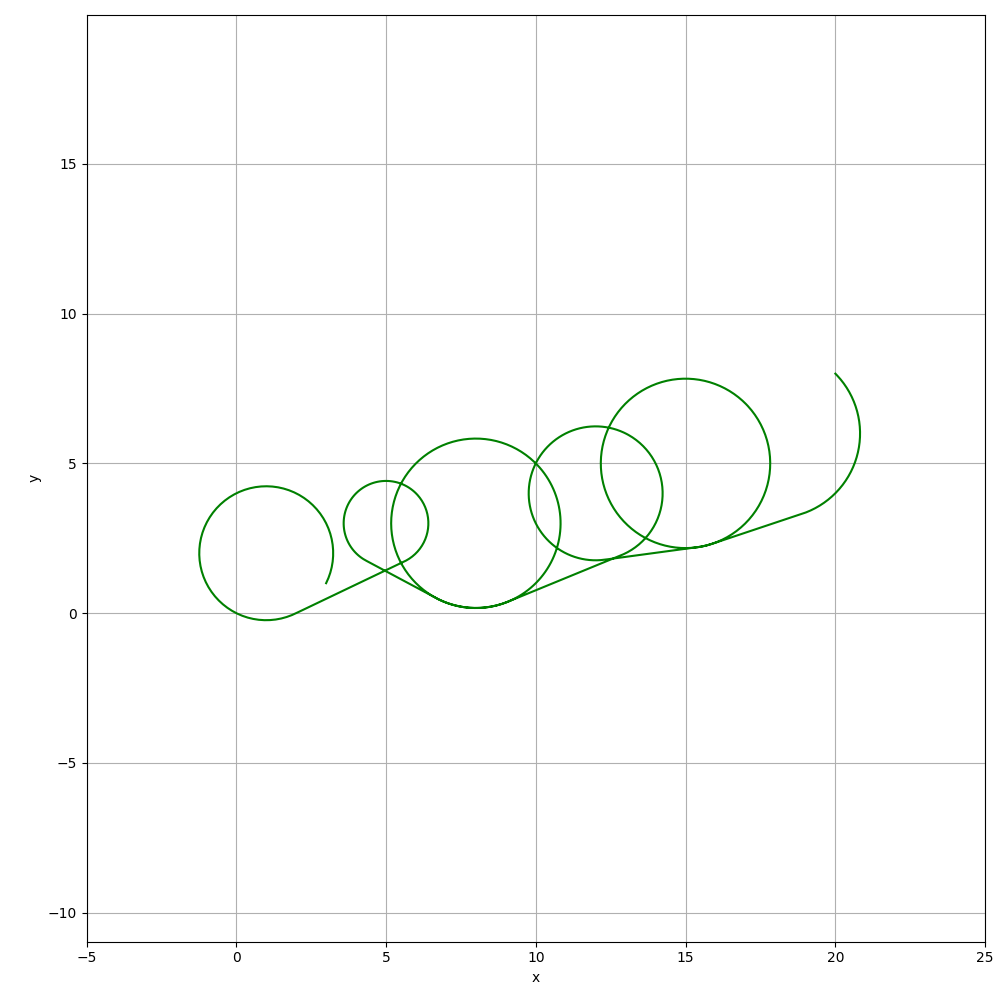
\includegraphics[width=1.0\linewidth]{Plots/CoverPlot.png}
\newpage
\end{center}



\section{The Context}

\section{The Data}

\section{The Encoding}

\section{Preliminary Definitions}
\textbf{AVOID STACKED HEADINGS}

\subsection{Data Points and their Indices}
Our system compresses a sequence of data points on-the-fly, by processing each one as it arrives. Let \(p\) be an arbitrary data point handled by the system. Let its first coordinate \(t_p\) be its time value, and let its second coordinate \(s_p\) be its sample value:

\[ p = (t_p, s_p) \]

The sample value \(s_p\) is a scalar; it is an individual measurement of some real-world quantity reported by a data source (sensor, gauge, etc.).

The time value \(t_p\) is the timestamp associated with the sample, which is generally the time at which the sample was collected. The system supports any unit of time (miliseconds, seconds, minutes, etc.), as well as fixed or variable intervals between readings. The system does \textit{not} require an initial time value of \(t = 0\). Time values are expected to be monotonically increasing, which means that time must not go backwards.

A zero-based index is assigned to each data point when it is received by the system. Let \(\mu_p\) be the index of data point \(p\).
The index for the first data point of the stream is \(\mu = 0\), the index for the second point is \(\mu = 1\), and so on. If the total count of data points received so far is \(n\), then the index of the most recent point is \(\mu = n-1\). Each index is permanently associated only with assigned data point. All indicies are unique.

\subsection{Overview of Data Representations}
There are three possible representations for any given data point in the system: \textit{actual}, \textit{encoded} and \textit{decoded}.
\subsubsection{Actual Data Point Representation}
We refer to the raw, uncompressed representation of the time and sample values of a data point as their actual time and actual sample values, respectively.
For data point \(p\), let its actual time value be \(t_{p_{actual}}\), and let its actual sample value be \(s_{p_{actual}}\). Actual data point values are exactly equal to the values that were originally reported from the data source.

\subsubsection{Compressed and Decompressed Data Point Representations}
After the system compresses data point \(p\), then \(p\) can be represented by its index \(\mu_p\) and the coefficents of the two associated fitted curves. \newline

\textbf{\thesubsubsubsection{    Time Piecewise Polynomial (TPP)}} /par
The Time Piecewise Polynomial (TPP) is the piecewise curve used to compress the time values of all data points. The independent variable of the TPP is the index \(\mu\) of the data point. The dependent variable of the TPP is the time \(t\) of the data point.

Let \(k_T\) be the degree of all fitted curves in the Time Piecewise Polynomial.

Let the coefficents of each fitted curve Time Piecewise Polynomial denoted as:

\[ [ \tau_{i_{0}}, \tau_{i_{1}} ] \]


Let \(n_T\) be current count of all fitted curves in the Time Piecewise Polynomial.

Where \(i\) is the smallest index \(\mu\) whose data point is represented by the same curve. The linear term coefficent is \(\tau_{i_{0}}\), and the constant term coefficent is \(\tau_{i_{1}}\). Thus, the decoded representation of the point with index \(\mu_k\) could be calculated by the equation:

\[ T_i(\mu) = \tau_{i_{0}}\mu + \tau_{i_{1}} \]


\subsection{Decoded Data Point Representation}



\subsection{If and When Actual Data Points can be Discarded}
\label{subsec:when_can_discard_point_coords}
\textbf{(This section was written in a legacy context...back when the plan was to use the intermediate matrices approach.)}
The y value (if not also the t value) of a data point can be discarded as soon as the intermediate matrices used to make the segment’s curve fit have been constructed. But when exactly is that? The current open segment must accumulate at least k+1 data points before we can attempt the initial k-degree polynomial fit for that segment. So, in general, the actual point coordinates will be retained until the current open segment has at least k+1 data points. The primary exception is for when the data stream ends while the open segment has k or fewer points. In this case, no k-degree polynomial fit can be attempted on this segment. (See also: \ref{subsec:close_the_final_segment})


\section{Lossiness}

\section{The Decoding}

\section{Parameters of the System}
1D time series data: (time, atmospheric pressure).
Compression is lossy.
Our system is based on best-fit curves interpolation: the method of least squares.
Our system is not "axis-agnostic:" when measuring error, we measure the distance from each actual data value to its fitted curve parallel with the vertical axis.

\section{Compression Ratio}
During an actual time-series streaming data scenario, there would be no complete, uncompressed, "before" data file on disk to compare our compression results to. For the purpose of this project, we do begin with a complete, uncompressed input data file that we use to simulate the streaming data scenario: we operate on each actual data point from the input sequentially, one at a time, without "peeking" at points that "haven't arrived yet." Our compression ratio comparisons are based on how large the complete, uncompressed data file would be on disk \textit{if} it were stored, which it would not be in practice.



\section{Demonstrations}
(since our system is lossy, we must show “before and after” photos)

\section{Limitations}
\subsection{Exceptional Cases}

\subsection{Determinism of Results}
Recall that a closed segment is a segment whose polynomial fit has been finalized, that is, the segment will not accept any additional data points. If you use a t value corresponding to a closed segment for querying its y value, the result will be deterministic: it will evaluate to the same y value every time. Of course, it is not expected to be exactly equal to the actual y value from the original point.

Recall that the current open segment is the segment whose polynomial is *not necessarily* finalized, it is the segment which *may* receive more points before it is ultimately closed. If you use a t value corresponding to the current open segment for querying its y value, the result will *not* be deterministic: it may or may not exactly match the y value from previous or subsequent queries of that same t.
If the curve for the open segment is re-fit, as long as the resulting residual error is within epsilon, that re-fit will become the new fit for the current open segment. It is possible for the curve of the open segment to be re-fit every time a new data point is added. This could happen *many* times before the segment is closed.

Hopefully this isn’t an issue for the client, as all of the queried y values will be estimates anyway and the re-fit had to meet the residual error bound requirement in order to be accepted in the first place. Still, the non-deterministic nature of y lookups in the open segment is something to be aware of while using this system. Any code that would rely on deterministic y value lookups within the open segment would be incorrect.


\section{Further Ideas}


\section{PYTHON DEVELOPMENT TO DO LIST}

\subsection{Size Comparison (for Compression section)}
Initially, compare theoretical data sizes in bytes between the raw data and the encoded/compressed data (coefficients for the k polynomial of each segment, start time t of each segment, any other metadata required to decode/decompress).

Eventually, actually write the data to file to compare file sizes on disk. Suggest using a simple text file with spaces and newlines as delimiters, rather than doing more elaborate compression on top of our basic scheme. There is enough complexity in our system as it is.
We could mention ideas for further compression in the “Possible Extensions” section.

\subsection{Time-Delay Simulation}
Visually simulate the time-delay of the incoming stream of data. This would be for the purpose of animating the curve fit over time as data points arrive and visually growing the overall piecewise curve for the data set as it accumulates.

Possibly matplotlib animation features? I couldn’t get them to work. Plotly also looked promising, but it seems to require webserver setup, etc.
I will defer to the judgment of whomever works on this.


\subsection{Close the Final Segment}
\label{subsec:close_the_final_segment}
When the data stream ends, formally close the current open segment. Current best idea is to not compress these points at all and simply store the actual t and y values to be appended to the end of the decompressed data. (See also \ref{subsec:when_can_discard_point_coords})

\subsection{Pressure Units OK?}
Do the units of pressure shown on the plot and in the comments correspond to the numerical pressure values in the data set? I suspect they may not.


\subsection{Data Values with Frequency Greater than One}
Clearly, any given property value may appear any number of times in the data set. (Example.) Further, equal property values generally will not occur at adjacent values of mu, nor will they be associated with any particular value of t.
But what about time values? Thanks to our parametric definition, there is no reason to restrict encoding multiple data points with the same time value. However, the Time Piecewise Polynomial is designed with the monotonically increasing property of time in mind, so for any times that appear in the data set more than once, we will require that they appear at consecutive values of mu. 
(We are leveraging the fact that time is monotonically increasing: time never goes backwards.)



\begin{figure}
    \centering
    \caption*{Progression Examples for the Representation of an Individual Data Point}
    \includegraphics[width=1.0\textwidth]{NoCorner.png}
    \caption{A non-exhaustive selection of possible scenarios for the progression of representation forms of an individual data point \((t,y)\)}
    \label{fig:does_not_create_a_corner}
\end{figure}


\newpage
\newpage
\mbox{} % This puts an empty box on the page, making LaTeX treat it as having content.



\section{The Motivation}
\label{sec:the_motivation}
There are countless practical applications of collecting data over time and storing it for later use. An application may use time-series data: a set of points where each point consists of some value and its associated time.

\subsection{More Data Than Can Be Stored}
\label{subsec:practical_applications}
For some applications, time series data may be collected frequently, potentially many times per second. \textbf{(Give example.) } Time-series data may also be collected over the span of a long time, possibly over the course of months or years. \textbf{(Example). } Some time-series data may be both collected very frequently and for a very long time. \textbf{Example.} In these types of situations, it may be impractical to store the value and time of each data point with perfect accuracy: the data may exceed the available storage. This is especially relevant in embedded applications where there is little local storage available and no (or no reliable) network connection.

\subsection{Selectively Discard Unnecessary Accuracy}
\label{subsec:unnecessary_accuracy}
Further, depending on the application, perfect accuracy of times and/or values may simply be unnecessary, so the extra space taken to store perfectly accurate values would be a waste of valuable storage resources. \textbf{(Example)}

\section{The Idea: Best-Fit Piecewise Interpolating Polynomials}
\label{sec:the_idea}
As an alternative to storing exact time and value data for each point in a time-series data stream, we propose a highly adjustable, on-the-fly compression system using best-fit piecewise interpolating polynomials.

\subsection{Deciding What to Fit}
\textbf{AVOID STACKED HEADINGS: put some intro text here}
\subsubsection{Using Best-Fit With a Common Approach}
A common approach to storing time-series data points is to record time as the first coordinate (the "x") and to record the data value as the second coordinate (the "y"). Best-fit piecewise polynomials \textit{could} be used to encode the data given this approach. However, since time would be the independent variable, time data with perfect accuracy while reducing the accuracy of what is presumably the more precious half of the information: the data values being collected!

\subsubsection{Fitting Time and Value Data Separately}
\textbf{TODO: go back and adjust wording so that the use of the term "point" is unambiguous in all contexts. Is a point a \((t,v)\) time-to-value point, a \((\mu,t)\) $\mu$-to-\(t\) point, or a \((\mu,v)\) $\mu$-to-\(v\) point?}

As an alternative, we encode the two parts of the input data readings separately: times are encoded by the \textit{Time Piecewise Polynomial} and values are encoded by the \textit{Value Piecewise Polynomial}. For both piecewise polynomials, let the independent variable $\mu$ be the zero-based index of each successive data sample, that is, the first data sample corresponds to $\mu = 0$, the second data sample corresponds to $\mu = 1$, and so on.

For the points interpolated by the Time Piecewise Polynomial, let the dependent variable \(t\) be the time of the data sample with corresponding index $\mu$.

For the points interpolated by the Value Piecewise Polynomial, let the dependent variable \(v\) be the value of the data sample with corresponding index $\mu$.

Downsides of this approach:
For live access to encoded data, 




Our goal is to use a set of points to generate an aesthetically pleasing curve consisting only of circle arcs and line segments. Our method interpolates between points by interpreting pairs of points as defining circles, then drawing arcs of those circles and connecting those arcs with line segments at tangent points.

\newpage
\newpage
\mbox{} % This puts an empty box on the page, making LaTeX treat it as having content.


\subsection{Interpreting the Input Data Set}
For an input data set of \( n \) points, let the \( \frac{n}{2} \) pairs of points be:

\[ P_0, P_1, \ldots, P_{n-2}, P_{n-1} \]

Note that \( n \) must be an even number. Let the even-indexed points be the "control" points, the center points of the circles:

\[ P_0 = C_0, P_2 = C_1, \ldots, P_{n-2} = C_{\frac{n}{2}-1} \]

Let the odd-indexed points be the "anchor" points, the points on the circumference of the circles:

\[ P_1 = A_0, P_3 = A_1, \ldots, P_{n-1} = A_{\frac{n}{2}-1} \]

%\vspace{0.2cm} % Adjust the vertical space as needed

\begin{figure}[!h]
\centering
\begin{tikzpicture}
    % Draw the circle
    \draw (0,0) circle (2cm);
    
    % Label the center
    \draw (0,0) node[circle,fill,inner sep=1.5pt,label=below:$C_i$] {};
    
    % Draw a point on the circumference
    \draw (135:2cm) node[circle,fill,inner sep=1.5pt,label=above left:$A_i$] {};
\end{tikzpicture}
\caption{Pairs of points in from the input data set represent a circle.}
\label{fig:pairs_of_points_define_a_circle}
\end{figure}

%\vspace{0.2cm} % Adjust the vertical space as needed

Each pair of points \( \{C_i, A_i\} \) define a circle, as shown in Fig. \ref{fig:pairs_of_points_define_a_circle}. The \( \frac{n}{2} \) pairs of points define \( \frac{n}{2} \) circles. A minimum of four points defining two circles (\( n \geq 4 \)) is required to use our method.

\subsubsection{Adjacent Circles Must be Disjoint}
Circles that are adjacent \textit{in the input data list} must be disjoint, that is, they must not intersect or be one inside the other. Circle \( \{C_i, A_i\} \) must be disjoint from circle \( \{C_{i-1}, A_{i-1}\} \), and also disjoint from circle \( \{C_{i+1}, A_{i+1}\} \). Circle \( \{C_i, A_i\} \) may or may not be disjoint from any other circle in the input data set. Note that there are only disjoint-ness requirements for circles based on their positions in the input data set, not based on any geometric relationship between them.


\subsection{A Parametric, Piecewise Curve}
\label{subsec:definition_of_curve}
Let the final curve be defined by a parametric piecewise function of $t$:
\begin{equation}
    \label{eq:O(t)}
\overrightarrow{O}(t) = \overrightarrow{O}_{\lfloor t \rfloor}(t - \lfloor t \rfloor) = \begin{cases}
S_0(t) & \text{for } 0 \leq t < 1, \\
L_1(t - 1) & \text{for } 1 \leq t < 2, \\
R_2(t - 2) & \text{for } 2 \leq t < 3, \\
S_3(t - 3) & \text{for } 3 \leq t < 4, \\
L_4(t - 4) & \text{for } 4 \leq t < 5, \\
R_5(t - 5) & \text{for } 5 \leq t < 6, \\
\vdots & \\
S_{\frac{3n}{2}-6}(t - \frac{3n}{2}-6) & \text{for } \frac{3n}{2}-6 \leq t < \frac{3n}{2}-5, \\
L_{\frac{3n}{2}-5}(t - \frac{3n}{2}-5) & \text{for } \frac{3n}{2}-5 \leq t < \frac{3n}{2}-4, \\
R_{\frac{3n}{2}-4}(t - \frac{3n}{2}-4) & \text{for } \frac{3n}{2}-4 \leq t < \frac{3n}{2}-3, \\
A_{\frac{n}{2}-1} & \text{for } t = \frac{3n}{2}-3
\end{cases}
\end{equation}

Where:
\begin{itemize}
    \item $n$ is the number of points in the input data set
    \item $\lfloor \cdot \rfloor$ is the floor function, which rounds down to the largest integer value less than or equal to the variable inside. Examples: $\lfloor 2.0 \rfloor = 2.0$, $\lfloor 2.6 \rfloor = 2.0$.
    \item The initial direction of arc travel around circle $\{C_0, A_0\}$ starting from $A_0$ is defined to be counter-clockwise.
    \item $S$ is the "Sender" function that gives the portion of the $\{C_i, A_i\}$ circle's arc which connects its anchor point $A_i$ to its tangent "sending" point $T_{iS}$. The sending point is the point on the circle tangent to the line segment\footnote{For any two disjoint circles, there exist four tangent lines: two internal tangent lines and two external tangent lines (see Fig. \ref{fig:external_tangents_only}). For our curve, we will consider only external tangent lines.} connecting circle $\{C_i, A_i\}$ to circle $\{C_{i+1}, A_{i+1}\}$ such that the resulting curve has no corner, as seen in Fig. \ref{fig:does_not_create_a_corner}.
    Note that the counter-clockwise direction of arc travel determines which of the tangent points on circle $\{C_i, A_i\}$ will be the correct tangent sending point $T_{iS}$, that is, the one that does not create a corner. Note also that defining the travel direction for the first sending arc to be counter-clockwise also defines travel direction for all arcs in the curve to be counter-clockwise.
    \item $L$ is the "Line" function that gives the line segment connecting the tangent sending point $T_{iS}$ on circle $\{C_i, A_i\}$ to the tangent receiving point $T_{iR}$ on circle $\{C_{i+1}, A_{i+1}\}$.
    \item $R$ is the "Receiver" function that gives the portion of the $\{C_{i+1}, A_{i+1}\}$ circle's arc that connects the tangent receiving point $T_{iR}$ to its anchor point $A_{i+1}$.
\end{itemize}

\begin{figure}
    \centering
    \includegraphics[width=1.0\textwidth]{NoCorner.png}
    \caption{The correct tangent sending point $T_{iS}$ is the one that does not create a corner.}
    \label{fig:does_not_create_a_corner}
\end{figure}

Fig. \ref{fig:SLRExample} shows an example resulting curve with the $S$ "Sending" function plots shown in green, the $L$ "Line" plots shown in blue, and the $R$ "Receiver" plots shown in orange.
\begin{figure}
    \centering
    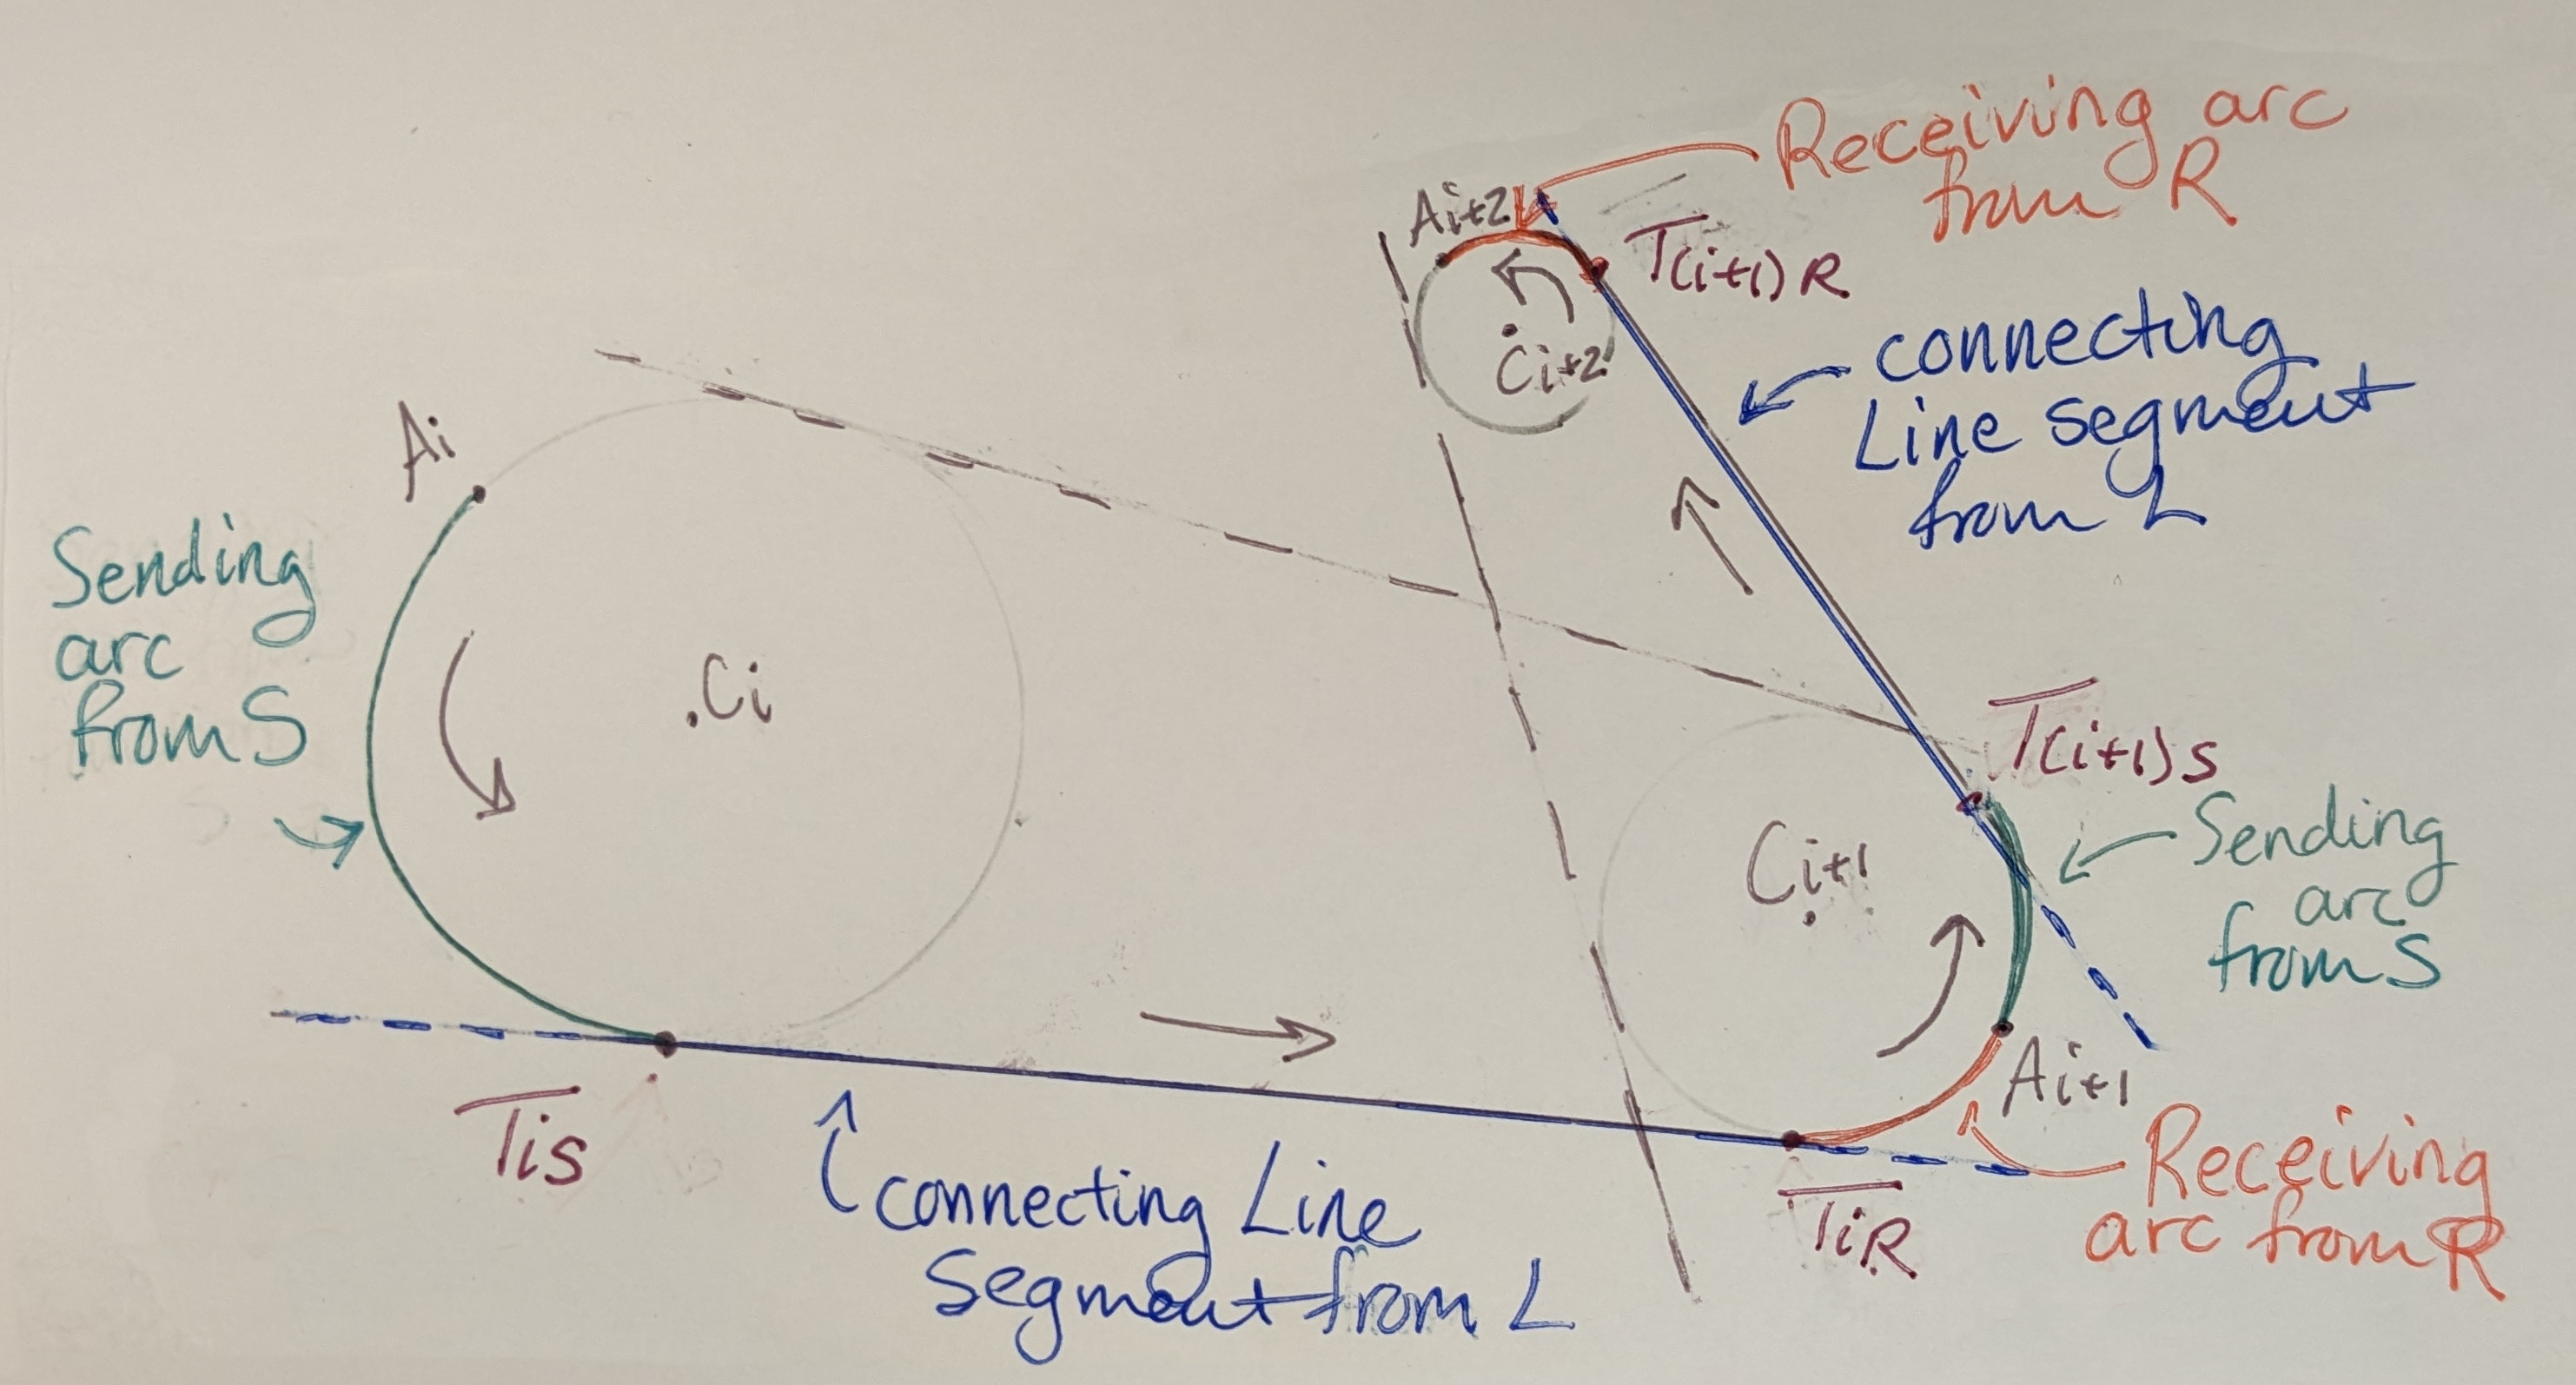
\includegraphics[width=1.0\textwidth]{FigureXExampleOfSLR_Cropped.png}
    \caption{Example curve showing $S$ "Sending" function plots (green), $L$ "Line" plots (blue), and $R$ "Receiver" plots (orange)}
    \label{fig:SLRExample}
\end{figure}

\begin{figure}[htbp]
    \centering
    %\vspace{0.2cm} % Adjust the vertical space as needed
    \begin{tikzpicture}
        % Draw the larger circle
        \draw (0,0) circle (2cm);
        % Draw the smaller circle
        \draw (5,0) circle (1cm);
        
        
        % Tangency points on the larger circle (for reference)
        \coordinate (T1) at (0.4, 1.96);
        \coordinate (T2) at (0.4, -1.96);
        
        % Tangency points on the smaller circle (for reference)
        \coordinate (T3) at (5.2, 0.98);
        \coordinate (T4) at (5.2, -0.98);
        
        % Draw the tangent lines (for reference)
        \draw[blue] (T1) -- (T3);
        \draw[blue] (T2) -- (T4);
    
        % Internal tangency points
        \coordinate (T5) at (1.2, 1.6);
        \coordinate (T6) at (1.2, -1.6);
        \coordinate (T7) at (4.4, 0.8);
        \coordinate (T8) at (4.4, -0.8);
        
        % Draw the internal tangent lines in red
        \draw[red] (T5) -- (T8);
        \draw[red] (T6) -- (T7);
    \end{tikzpicture}
    \caption{The tangent lines of two disjoint circles: two internal tangent lines (red) and two external tangent lines (blue). Our curve considers only external tangent lines.}
    \label{fig:external_tangents_only}
\end{figure}
%\vspace{0.2cm} % Adjust the vertical space as needed
\subsubsection{Interpretation and Usage of Parameter Variable $t$}
The range of values that can be used with (\ref{eq:O(t)}) $\overrightarrow{O}(t)$ is $0 \leq t \leq \frac{3n}{2}$. The first point of the curve $P_1 = A_0$ is plotted by function $S_0$ when $t = 0$. The final point of the curve $P_{n-1} = A_{\frac{n}{2}-1}$ is plotted directly when $t = \frac{3n}{2}$, without using any of the $SLR$ functions.
Table \ref{tab:n_t_and_SLR_relationship} gives examples showing the relationship between $n$, the maximum value of $t$, and the indices of all $SLR$ functions (and the final $A$ point) of the piecewise curve definition.

\begin{table}[htbp]
    \centering
    \begin{tabular}{|c|c|c|c|}
        \hline
        Input data count & \multicolumn{1}{c|}{\begin{tabular}[t]{@{}c@{}}
            $n = 4$ points \\
            $\frac{n}{2} = 2$ circles
        \end{tabular}} &
        \multicolumn{1}{c|}{\begin{tabular}[t]{@{}c@{}}
            $n = 6$ points \\
            $\frac{n}{2} = 3$ circles
        \end{tabular}} &
        \multicolumn{1}{c|}{\begin{tabular}[t]{@{}c@{}}
            $n = 8$ points \\
            $\frac{n}{2} = 4$ circles
        \end{tabular}} \\
        \hline
        All piecewise functions & \multicolumn{1}{|c|}{\begin{tabular}[t]{@{}c@{}}
            $S_0$ \\
            $L_1$ \\
            $R_2$ \\
            $A_1$ 
        \end{tabular}} &
        \multicolumn{1}{|c|}{\begin{tabular}[t]{@{}c@{}}
            $S_0$ \\
            $L_1$ \\
            $R_2$ \\
            $S_3$ \\
            $L_4$ \\
            $R_5$ \\
            $A_2$ 
        \end{tabular}} &
        \multicolumn{1}{|c|}{\begin{tabular}[t]{@{}c@{}}
            $S_0$ \\
            $L_1$ \\
            $R_2$ \\
            $S_3$ \\
            $L_4$ \\
            $R_5$ \\
            $S_6$ \\
            $L_7$ \\
            $R_8$ \\
            $A_3$ 
        \end{tabular}} \\
        \hline
        Range of possible $t$ values & \multicolumn{1}{|c|}{\begin{tabular}[t]{@{}c@{}}
            $0 \leq t \leq \frac{3n}{2}-3$ \\
            \hspace{1.5em}$\leq \frac{3 \cdot 4}{2}-3$ \\
            $0 \leq t \leq 3$
        \end{tabular}} &
        \multicolumn{1}{|c|}{\begin{tabular}[t]{@{}c@{}}
            $0 \leq t \leq \frac{3n}{2}-3$ \\
            \hspace{1.5em}$\leq \frac{3 \cdot 6}{2}-3$ \\
            $0 \leq t \leq 6$
        \end{tabular}} &
        \multicolumn{1}{|c|}{\begin{tabular}[t]{@{}c@{}}
            $0 \leq t \leq \frac{3n}{2}-3$ \\
            \hspace{1.5em}$\leq \frac{3 \cdot 8}{2}-3$ \\
            $0 \leq t \leq 9$
        \end{tabular}} \\
        \hline
    \end{tabular}
    \caption{Comparison of three curve scenarios with point count, circle count, piecewise function instantiation, and corresponding range of possible $t$ values. }
    \label{tab:n_t_and_SLR_relationship}
\end{table}

\subsubsection{Overlapping Arcs}
Consider the scenario where the position of anchor point $A_{i+1}$ on circle $\{C_{i+1}, A_{i+1}\}$ causes the receiving arc (going from $T_{iR}$ to $A_{i+1}$) to overlap with the sending arc (going from $A_{i+1}$ to $T_{(i+1)S}$). In this scenario, the entire $\{C_{i+1}, A_{i+1}\}$ circle will be plotted. Further, some of circle $\{C_{i+1}, A_{i+1}\}$ will be plotted twice: first by the $R$ function, then again by the $S$ function.

Such overlapping of receiving and sending arcs does not affect which point will become the $T_{(i+1)S}$ tangent sending point for circle $\{C_{i+1}, A_{i+1}\}$. The correct tangent sending point is determined only by the direction of arc travel, which is counterclockwise for all arcs in the curve.

\section{The Computation}
\label{sec:the_computation}
The computation of $SLR$ functions that are adjacent in the piecewise definition of (\ref{eq:O(t)}) $\overrightarrow{O}(t)$ are closely related, so we will discuss them as a group. Further, the computation of an $SLR$ group uses \textit{only} four points from the input data set: the two that define the circle of the sending arc and the two that define the circle of the receiving arc. No results from computation of other $SLR$ groups are required.

\subsection{Subscripts, Indices, Conversion and Local Function Scope}
In an effort to make the computation process more user-friendly, we will make a case for using a local function scope for the computation of an isolated $SLR$ function group.
\subsubsection{Conversion of $SLR$ Function Subscripts to Circle Indices}
\label{subsubsec:SLR_subscript_conversion}
During the computation, we will use the subscript of the called $SLR$ function to look up the corresponding points of the sending circle $\{C_i, A_i\}$ and the points of the receiving circle $\{C_{i+1}, A_{i+1}\}$. The conversion from $SLR$ function subscripts to circle indices is shown in Table \ref{tab:my_conversion_from_SLR_subscript_to_circle_subscripts}, with an example conversion worked out in Table \ref{tab:my_conversion_from_SLR_subscript_to_circle_subscripts_EXAMPLE}.

Note that all three functions in an $SLR$ group share the same $\{C_i, A_i\}$ circle for the sending arc and the same $\{C_{i+1}, A_{i+1}\}$ circle for the receiving arc.

The complexity of this scheme serves to ensure that the range of $t$ values passed into any $SLR$ function is $0 \leq t < 1$. To make that happen, we define the subscript of the first $S$ function to be $0$, and the subscript of each following $SLR$ piecewise function to be one greater that the subscript of the previous function.

\begin{table}[h]
\centering
\begin{tabular}{|c|c|c|}
\hline
$\text{SLR Function Called}$ & $\text{Circle of Sending Arc}$ & $\text{Circle of Receiving Arc}$ \\
\hline
$S_u$ & $\{C_\frac{u}{3}, A_\frac{u}{3}\}$ & $\{C_\frac{u}{3}, A_\frac{u}{3}\}$\\
$L_v$ & $\{C_\frac{v-1}{3}, A_\frac{v-1}{3}\}$ & $\{C_\frac{v+2}{3}, A_\frac{v+2}{3}\}$\\
$R_w$ & $\{C_\frac{w-2}{3}, A_\frac{w-2}{3}\}$ & $\{C_\frac{w+1}{3}, A_\frac{w+1}{3}\}$\\
\hline
\end{tabular}
\caption{Formulas for looking up the circles of the sending and receiving arcs based on $SLR$ function subscript.}
\label{tab:my_conversion_from_SLR_subscript_to_circle_subscripts}
\end{table}

\begin{table}[h]
\centering
\begin{tabular}{|c|c|c|}
\hline
$\text{SLR Function Called}$ & $\text{Circle of Sending Arc}$ & $\text{Circle of Receiving Arc}$ \\
\hline
$S_6$ & $\{C_\frac{6}{3}, A_\frac{6}{3}\} = \{C_2, A_2\}$ & $\{C_\frac{6+3}{3}, A_\frac{6+3}{3}\} = \{C_3, A_3\}$\\
$L_7$ & $\{C_\frac{7-1}{3}, A_\frac{7-1}{3}\} = \{C_2, A_2\}$ & $\{C_\frac{7+2}{3}, A_\frac{7+2}{3}\} = \{C_3, A_3\}$\\
$R_8$ & $\{C_\frac{8-2}{3}, A_\frac{8-2}{3}\} = \{C_2, A_2\}$ & $\{C_\frac{8+1}{3}, A_\frac{8+1}{3}\} = \{C_3, A_3\}$\\
\hline
\end{tabular}
\caption{Example lookup of sending and receiving arcs based on $SLR$ function subscript.}
\label{tab:my_conversion_from_SLR_subscript_to_circle_subscripts_EXAMPLE}
\end{table}

\subsubsection{Symbols and Names Local to $SLR$ Group Computation}
\label{subsub:local_point_indices}
Since an $SLR$ group can be computed in complete isolation, local to its computation we will refer to the sending circle as $\{C_1, A_1\}$ and the receiving circle as $\{C_2, A_2\}$. Within this context, the $\{C_1, A_1\}$ and $\{C_2, A_2\}$ names effectively "shadow" the meaning of those names outside of the local context. The authors have lots of work expressed in this local naming scheme, and have opted to continue use of it here for sanity purposes. 

The computation of an $SLR$ group never refers to any points other than those defining its sending circle and receiving circle. The conversion from sub-subsection \ref{subsubsec:SLR_subscript_conversion} is the only connection between the computation of an $SLR$ group and any names from the input data set.

Within the context of computing an $SLR$ group, after the indices of the circles have been converted, we will refer to the $SLR$ functions without any subscript, as the purpose of the subscript is to facilitate identifying the indices of the points on which to operate.

Further, local to $SLR$ group computation, the parameter $t$ passed into an $SLR$ function will be the result of $t - \lfloor t \rfloor$ computed during the lookup (as shown in the piecewise function definition (\ref{eq:O(t)}) $\overrightarrow{O}(t)$ in subsection \ref{subsec:definition_of_curve}).

\subsection{Computation of an $SLR$ Function Group}
\label{subsec:SLR_group_computation}
Section \ref{sec:the_idea} described \textit{what} our method does as a whole: it gives the piecewise parametric function $\overrightarrow{O}(t)$ which plots the curve represented by the $\frac{n}{2}$ pairs of input points, supporting values in the range $0 \leq t \leq \frac{3n}{2}-3$.

This section details the computation of the $S$, $L$ and $R$ functions and substantiates their logic with principles from geometry and trigonometry.

\subsubsection{The Sending Function $S$}
\label{subsubsec:sending_function_S}
The sending function $S$ gives the arc on circle $\{C_1, A_1\}$ starting from known anchor point $A_1$ and ending at tangent "sending" point $T_{1S}$. For the correct external tangent line between circle $\{C_1, A_1\}$ and circle $\{C_2, A_2\}$, $T_{1S}$ is the tangent point that of that line to circle $\{C_1, A_1\}$.

We must find an expression for $T_{1S}$. To that end, we construct a diagram of geometric relationships between circle $\{C_1, A_1\}$ and circle $\{C_2, A_2\}$, as shown in Fig. \ref{fig:SLR_Primary}.

\begin{figure}
    \centering
    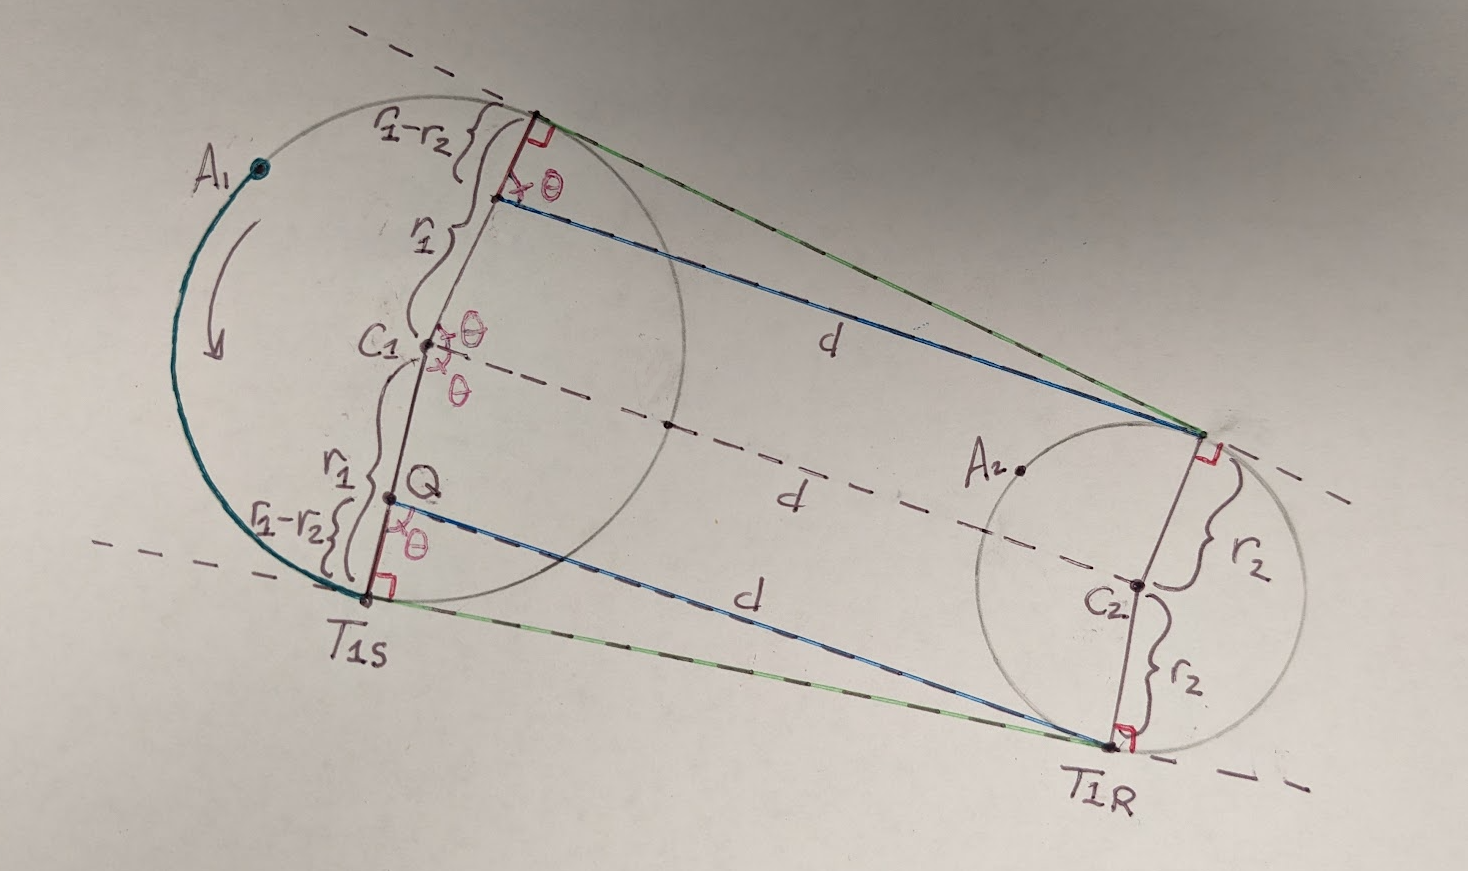
\includegraphics[width=1.0\textwidth]{SLRPrimary.png}
    \caption{Geometric relationships between circle $\{C_1, A_1\}$ and circle $\{C_2, A_2\}$.}
    \label{fig:SLR_Primary}
\end{figure}

\paragraph{Finding an expression for $T_{1S}$}
First, we draw the external tangent lines to the circles, and draw a line segment connecting circle center $C_1$ to tangent point $T_{1S}$. We note that the length of this line segment is equal to the radius of circle $\{C_1, A_1\}$. Let $r_1$ be the radius of circle $\{C_1, A_1\}$:

\begin{equation}
    \label{eq:r_1}
    r_1 = \sqrt{(A_1.x - C_1.x)^2 + (A_1.y - C_1.y)^2}
\end{equation}

We also note that the angle between the radius line segment and the tangent line is a right angle.

We draw a line segment connecting circle center $C_2$ to tangent point $T_{1R}$. We note that the length of this line segment is equal to the radius of circle $\{C_2, A_2\}$. Let $r_2$ be the radius of circle $\{C_2, A_2\}$:

\begin{equation}
    \label{eq:r_2}
r_2 = \sqrt{(A_2.x - C_2.x)^2 + (A_2.y - C_2.y)^2}
\end{equation}

We draw a line segment connecting circle center $C_1$ to circle center $C_2$. We note that the length of this line segment is equal to the distance between the centers of the circles. Let $d$ be the distance between circle $\{C_1, A_1\}$ and circle $\{C_2, A_2\}$:

\begin{equation}
    \label{eq:d}
    d = \sqrt{(C_2.x - C_1.x)^2 + (C_2.y - C_1.y)^2}
\end{equation}

For the line segment connecting $C_1$ to $C_2$, we draw a line segment parallel to it from $T_{1R}$ towards circle $\{C_1, A_1\}$. The line segment is of length $d$ and ends at a point on the radius line segment between $C_1$ and $T_{1S}$. Let this point be point $Q$.

We note that the angle between the $C_1$, $T_{1S}$ line segment and the $C_1$, $C_2$ line segment is equal to the angle between the $Q$, $T_{1S}$ line segment and the $Q$, $T_{1R}$ line segment. Let that angle be $\theta$.

We note that the length of the $Q$, $T_{1S}$ line segment is equal to $r_1 - r_2$.

We observe a right triangle where the hypotenuse is the $Q$, $T_{1R}$ line segment, the adjacent side to $\theta$ is the $Q$, $T_{1S}$ line segment, and the opposite side to $\theta$ is the $T_{1S}$,  $T_{1R}$ line segment. Using the Pythagorean theorem, we form this expression for $\theta$:

\begin{equation}
    \label{eq:theta}
    \theta = \arccos\left(\frac{r_1 - r_2}{d}\right)
\end{equation} 

We observe that point $T_{1S}$ is at angle $-\theta$ from the $C_1$, $C_2$ line segment. We note that in general, the $C_1$, $C_2$ line segment will not be aligned with the $x$ axis. Let $\alpha$ be the angle between the $C_1$, $C_2$ line segment and the $x$ axis:

\begin{equation}
    \label{eq:alpha}
    \alpha = atan2(C_2.y - C_1.y, C_2.x - C_1.x)
\end{equation}     

Where $atan2$ is the the two-argument arctangent function that returns the angle in the appropriate quadrant, taking into account the signs of both x and y.

Finally, we can express $T_{1S}$ in terms of known quantities:

\begin{equation}
    \label{eq:T_1S.x}
    T_{1S}.x = C_1.x + r_1 * cos(\alpha - \theta)
\end{equation}

\begin{equation}
    \label{eq:T_1S.y}
    T_{1S}.y = C_1.y + r_1 * sin(\alpha - \theta)
\end{equation}

That is, $T_{1S}$ is distance $r_1$ from $C_1$ at angle $-\theta$, where $\alpha$ is the angle between the $C_1$, $C_2$ line segment and the $x$ axis. 

\paragraph{Converting from Parameter $t$ to an Angle}
Recall that the purpose of the $S$ function is to draw the arc on  circle $\{C_1, A_1\}$ from $A_1$ to $T_{1S}$. Specifically, the $S(t)$ gives the point on that arc which corresponds to the parameter $t$, where $0 \leq t < 1$. $t = 0$ corresponds to $A_1$, while $t = 1$ would correspond to $T_{1S}$.\footnote{The $S$ function operates on $0 \leq t < 1$, so it stops just short of $T_{1S}$, rather. The $L$ function will handle $T_{1S}$.}

To do this interpolation, we need both $A_1$ and $T_{1S}$ expressed as angles.\footnote{Why bother to express $T_{1S}$ as $(x,y)$ coordinates in the first place? They will be useful when we get to discussing the $L$ function.} Let $\omega_{A1}$ be the angle of $A_1$ and let $\omega_{T1S}$ be the angle of $T_{1S}$:

\begin{equation}
    \label{eq:omega_A1}
    \omega_{A1} = atan2(A_1.y - C_1.y, A_1.x - C_1.x)
\end{equation}

\begin{equation}
    \label{eq:omega_T1S}
    \omega_{T1S} = atan2(T_{1S}.y - C_1.y, T_{1S}.x - C_1.x)
\end{equation} 

Finally, let $\Theta_S(t)$ be a function that gives the interpolated angle between $A_1$ and $T_{1S}$ for any $0 \leq t < 1$:

\begin{equation}
    \label{eq:Theta_S(t)}
    \Theta_S(t) = (1-t) \omega_{A1} + t \omega_{T1S}
\end{equation} 

\paragraph{Bringing it All Together: Sending Function $S$}
Now that we can convert directly from parameter $t$ to the corresponding angle on the sending arc, we can use that result to construct the $S$ piecewise function itself:

\begin{equation}
    \label{eq:S(t)}
    S(t) = C_1 + r_1 * ( cos( \Theta_S(t) ),  sin( \Theta_S(t) ) )
\end{equation} 

That is, for a given $t$, we return the point that is distance $r_1$ from point $C_1$ at the interpolated angle that corresponds to parameter $t$.


\subsubsection{The Line Segment Function $L$}
\label{subsubsec:line_segment_function_L}
The "Line" function $L$ gives the line segment connecting the tangent sending point $T_{1S}$ on circle $\{C_1, A_1\}$ to the tangent receiving point $T_{2R}$ on circle $\{C_2, A_2\}$.

Specifically, the $L$ function gives the point on the line that corresponds to parameter $t$, where $0 \leq t < 1$. $t = 0$ corresponds to $T_{1S}$, while $t = 1$ would correspond to $T_{1R}$.\footnote{The $L$ function operates on $0 \leq t < 1$, so it stops just short of $T_{1R}$. The $R$ function will handle $T_{1R}$.}

To do this interpolation, we need $T_{1S}$ and $T_{1R}$ expressed as $(x,y)$ coordinates. We already have $T_{1S}$ from sub-subsection \ref{subsubsec:sending_function_S}. Following the same logic and using the same $\alpha$ and $\theta$, we can express $T_{1R}$ in terms of all known quantities:

\begin{equation}
    \label{eq:T_1R.x}
    T_{1R}.x = C_2.x + r_2 * cos(\alpha - \theta)
\end{equation}

\begin{equation}
    \label{eq:T_1R.y}
    T_{1R}.y = C_2.y + r_2 * sin(\alpha - \theta)
\end{equation}

Now that we have the starting point of the line segment $T_{1S}$ and the ending point of the line segment $T_{1R}$, we can construct the $L$ piecewise function itself:

\begin{equation}
    \label{eq:L(t)}
    L(t) = T_{1S} + t * ( T_{1R} - T_{1S} )
\end{equation}

Interpreting $T_{1R} - T_{1S}$ as a vector from $T_{1S}$ to $T_{1R}$, $L(t)$ gives the point that is offset from the starting point $T_{1S}$ in the direction of $T_{1R} - T_{1S}$, scaled by $t$.

\subsubsection{The Receiving Function $R$}
The receiving function $R$ gives an arc on circle $\{C_2, A_2\}$ starting from tangent "receiving" point $T_{1R}$ and ending at known anchor point $A_2$. For the correct external tangent line between circle $\{C_1, A_1\}$ and circle $\{C_2, A_2\}$, $T_{1R}$ is the tangent point of the line to circle $\{C_2, A_2\}$. 

Specifically, $R(t)$ gives the point on that arc which corresponds to the parameter $t$, where $0 \leq t < 1$. $t = 0$ corresponds to $T_{1R}$, while $t = 1$ would correspond to $A_{2}$.\footnote{The $R$ function operates on $0 \leq t < 1$, so it stops just short of $A_2$. The final point of the curve is plotted directly by the piecewise definition of $\overrightarrow{O}(t)$ without using any of the $SLR$ functions. }

We already have $T_{1R}$ from sub-subsection \ref{subsubsec:line_segment_function_L}, and $A_2$ is known. We need to express both $T_{1R}$ and $A_2$ as angles. Let $\omega_{T1R}$ be the angle of $T_{1R}$ and $\omega_{A2}$ be the angle of $A_2$:

\begin{equation}
    \label{eq:omega_T1R}
    \omega_{T1R} = atan2(T_{1R}.y - C_2.y, T_{1R}.x - C_2.x)
\end{equation}

\begin{equation}
    \label{eq:omega_A2}
    \omega_{A2} = atan2(A_2.y - C_2.y, A_2.x - C_2.x)
\end{equation}

Let $\Theta_R(t)$ be a function that gives the interpolated angle between $T_{1R}$ and $A_2$ for any $0 \leq t < 1$:

\begin{equation}
    \label{eq:Theta_R(t)}
    \Theta_R(t) = (1-t) \omega_{T1R} + t \omega_{A2}
\end{equation}

Now that we can convert directly from parameter $t$ to the corresponding angle on the sending arc, we can use that result to construct the $R$ piecewise function itself:

\begin{equation}
    \label{eq:R(t)}
    R(t) = C_2 + r_2 * (cos( \Theta_R(t) ), sin( \Theta_R(t) ))
\end{equation} 

That is, for a given $t$, we return the point that is distance $r_2$ from point $C_2$ at the interpolated angle that corresponds to parameter $t$.


\subsubsection{The Final Point $A_{\frac{n}{2}-1}$}
Outside the scope of any $SLR$ function, the final point of the curve $P_{n-1} = A_{\frac{n}{2}-1}$ is handled directly by the piecewise definition of $\overrightarrow{O}$ when $t = \frac{3n}{2}$. Note that this is the same point that final $R$ function did not handle because $t$ never reached $1$ within that context.

\section{The Results}
Figure \ref{fig:demo_sequences} shows the results of our method applied to the provided demonstration sequences of points. Since sequence 3 contained an odd number of points, it was not valid input to our method and is thus omitted.

\begin{center}
\begin{figure}[ht]
\centering
\begin{tabular}{cc}

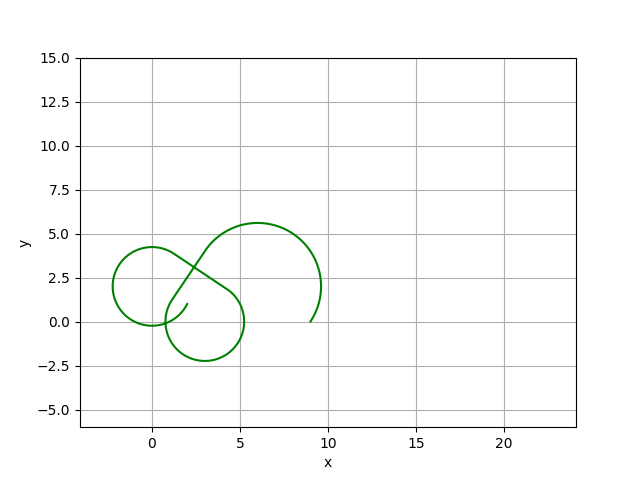
\includegraphics[width=0.4\linewidth]{Plots/DemoPlot1.png} &
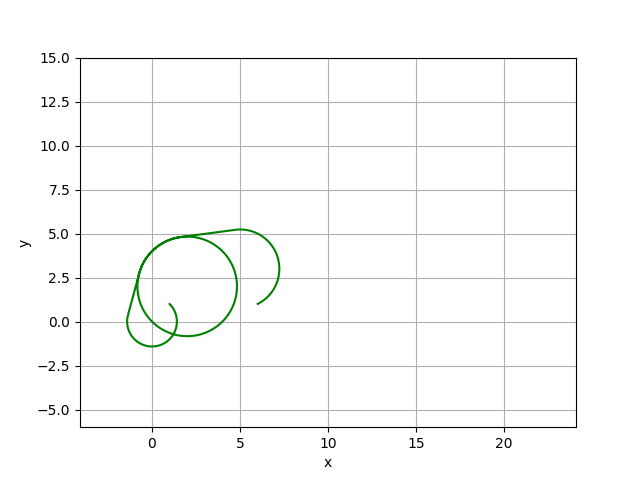
\includegraphics[width=0.4\linewidth]{Plots/DemoPlot2.png} \\
Sequence 1 & Sequence 2 \\ % Optional captions

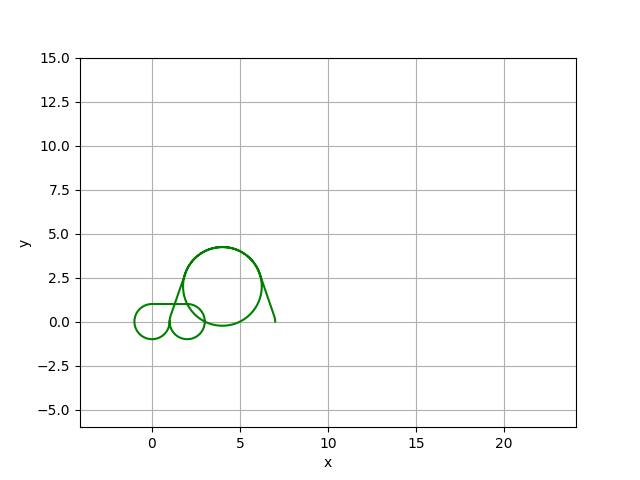
\includegraphics[width=0.4\linewidth]{Plots/DemoPlot4.png} &
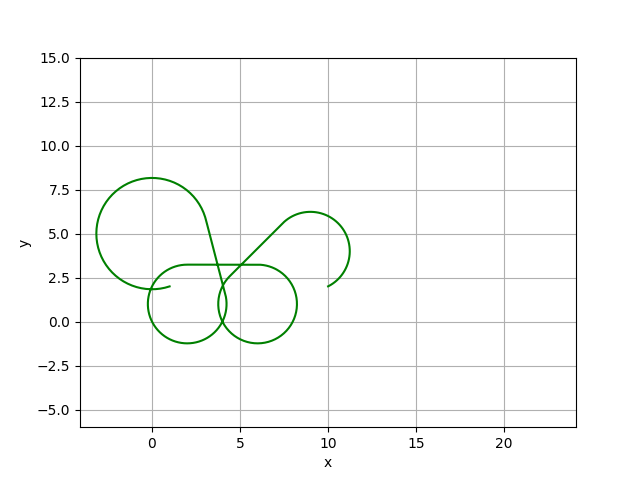
\includegraphics[width=0.4\linewidth]{Plots/DemoPlot5.png} \\
Sequence 4 & Sequence 5 \\ % Optional captions

\end{tabular}
\caption{Plots using our method on the required demonstration point sequences. (Sequence 3 has an odd number of points and is invalid input for our method.)}
\label{fig:demo_sequences}
\end{figure}
\end{center}

Figure \ref{fig:showcse_plots} shows some of our favorite results applying our method to sequences of points.

\begin{center}
\begin{figure}[ht]
\centering
\begin{tabular}{cc}

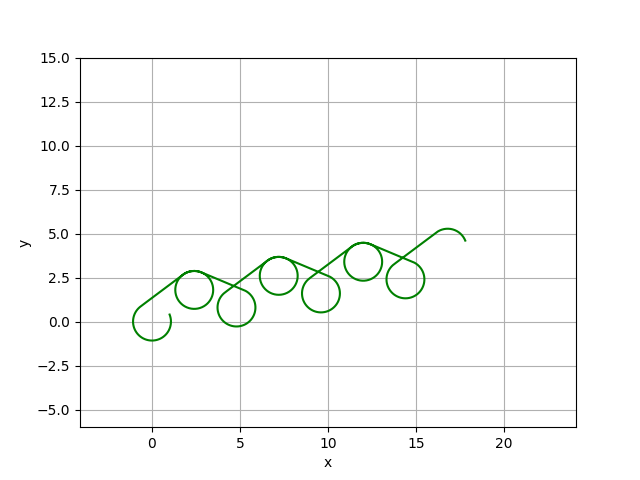
\includegraphics[width=0.4\linewidth]{Plots/ShowcasePlot1.png} &
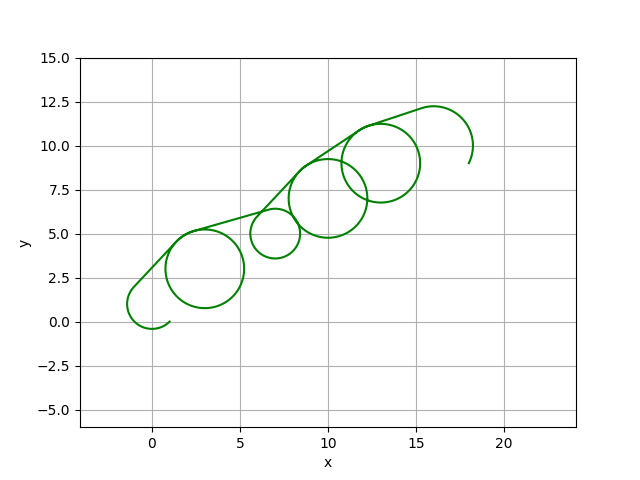
\includegraphics[width=0.4\linewidth]{Plots/ShowcasePlot4.png} \\
"Bouncy Biplane" & "Wavy Wonder" \\ % Optional captions

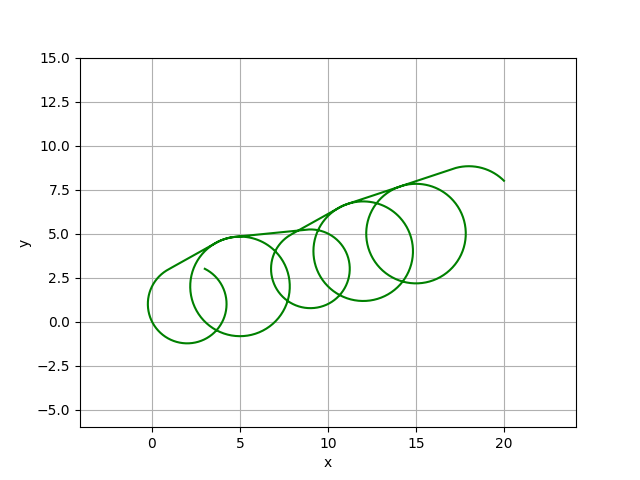
\includegraphics[width=0.4\linewidth]{Plots/ShowcasePlot2.png} &
\includegraphics[width=0.4\linewidth]{Plots/ShowcasePlot3.png} \\
"Contrary CanCan" & "Loopy Labyrinth" \\ % Optional captions

\end{tabular}
\caption{Showcase of four of our favorite results.}
\label{fig:showcse_plots}
\end{figure}
\end{center}


\section{Notable Curve Properties}
Our curve connects only the anchor points from the input data set, that is, the points on the edges of the circles. The control points serve only to define the center point of each circle. Thus, we have borrowed the point naming convention  of B\'ezier curves.

Our curve has no discontinuities or corners. It consists of only circle arcs connected by line segments at mutual tangent points. Since our curve is parametric and not a function of x, it can cross back across where it has already been on the x axis. Fulfilling our primary goal, a very nice property of our curve is that it flows pleasingly along its path even though it is made up entirely of simple geometric constructs: circle arcs and line segments. No calculus required.

Figure \ref{fig:axis_agnostic} demonstrates that our method is axis-agnostic. First, we show the results of our method applied to the points from Sequence 5. Then we show the results of our method applied to the points of Sequence 5 after they have been rotated $30^\circ$, $60^\circ$ and $180^\circ$ respectively. When the points of the figure are rotated, the output of our method rotates consistently with them.

As we discussed at the start of section \ref{sec:the_computation}, the computation of an $SLR$ group does not require information from the computation of any other $SLR$ group (such as derivatives). This is one significant advantage that our method has over interpolation methods such as Lagrange interpolation and splines: each $SLR$ group can be computed in isolation, there is no huge system of equations required to represent the curve as a whole.

\begin{center}
\begin{figure}
\centering
\begin{tabular}{cc}

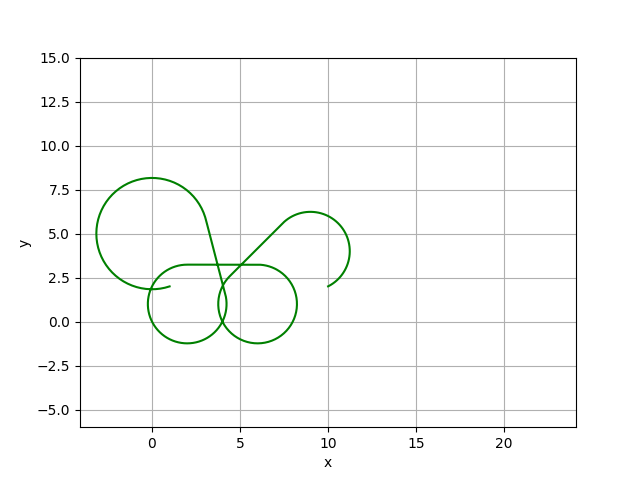
\includegraphics[width=0.4\linewidth]{Plots/DemoPlot5.png} &
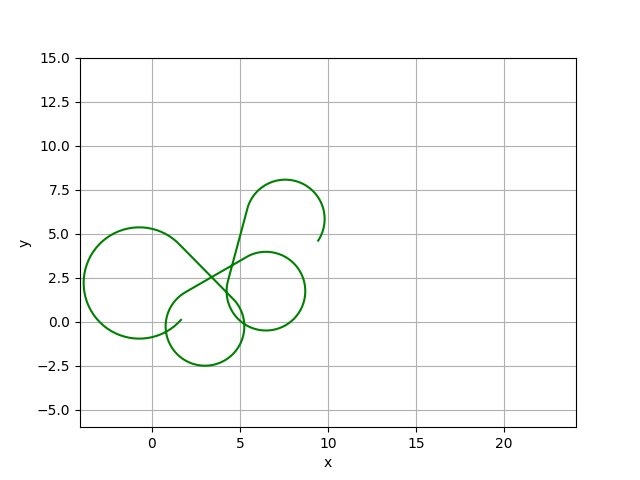
\includegraphics[width=0.4\linewidth]{Plots/DemoPlot5Rotate30.png} \\
No Rotation & Rotated $30^\circ$ \\ % Optional captions

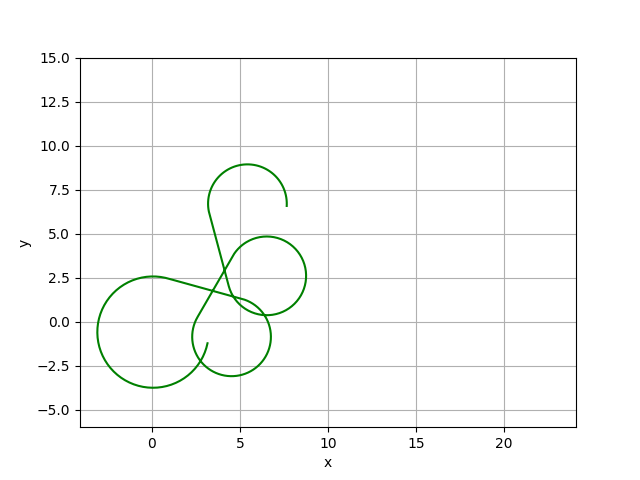
\includegraphics[width=0.4\linewidth]{Plots/DemoPlot5Rotate60.png} &
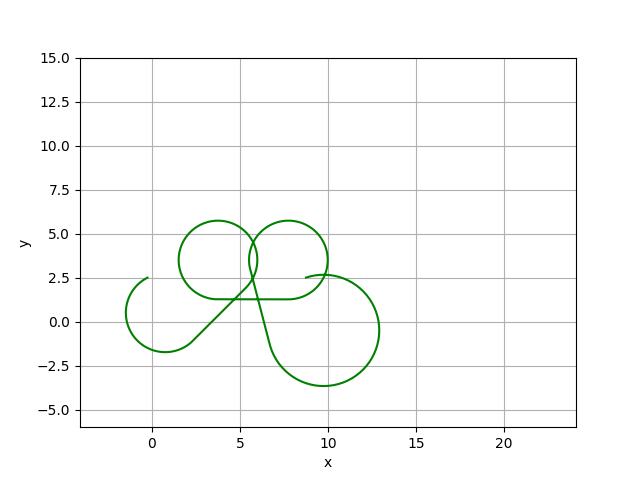
\includegraphics[width=0.4\linewidth]{Plots/DemoPlot5Rotate180.png} \\
Rotated $60^\circ$ & Rotated $180^\circ$ \\ % Optional captions

\end{tabular}
\caption{The points of Sequence 5 with no rotation, then $30^\circ$, $60^\circ$ and $180^\circ$ of rotation. Our method is axis-agnostic.}
\label{fig:axis_agnostic}
\end{figure}
\end{center}


\section{Limitations}
There are many prerequisites to using our method that are described in section \ref{sec:the_idea}. A given set of points is not generally valid input.

\subsection{Degenerate Arcs}
It is possible for an arc from a circle to be degenerate, that is, an arc that consists of a single point. If the line connecting circle $\{C_i, A_i\}$ and circle $\{C_{i+1}, A_{i+1}\}$ is the same line that connects circle $\{C_{i+1}, A_{i+1}\}$ with circle $\{C_{i+2}, A_{i+2}\}$, and the receiving tangent point on $\{C_{i+1}, A_{i+1}\}$ is also its anchor point $A_{i+1}$, then the arc of circle $\{C_{i+1}, A_{i+1}\}$ will be a degenerate arc: the single point $A_{i+1}$. For our purposes, this is not an issue since our goal is pleasing aesthetics.

However, if the circles in the dataset were to have some greater meaning, it may be important to deem invalid any input points that cause such degenerate arcs. The concern being that you would not be able to tell that circle $\{C_{i+1}, A_{i+1}\}$ existed just by looking at the curve.

\section{Further Ideas}
It would be easy to add support for clockwise arc rotation: just adjust equations (7), (8), (13), and (14) to use $(\alpha + \theta)$ instead of $(\alpha - \theta)$. This change corresponds to taking tangent point on the other external tangent line.

We think that allowing adjacent circles to intersect would be fine, but testing and documenting this was cut from the project for time. In our project, non-adjacent circles can already overlap, so we don't think that allowing adjacent circle intersection would make much of a difference in creative expression.

A circle being entirely contained within an adjacent circle, if permitted in the input data, should be fixed by deleting the contained circle. No internal or external tangent lines exist between a circle and another circle entirely contained within it.

Initially, we were interested in also using internal tangent lines. That is, the correct sending tangent point would be the one on the first tangent line that does not create a corner in the curve. Sometimes an external tangent line would be chosen and sometimes an internal tangent line would be chosen. This would create a conditional in the math and eliminates the advantage of $SLR$ group computation being isolated from other $SLR$ groups. Specifically, if an internal tangent line is taken from one circle to another, then the travel orientation (clockwise or counterclockwise) will swap at the start of the arc on the receiving circle. The result would give more opportunities for visual appeal, but it would also increase the complexity of our method quite a bit.

\end{document}
